% N.B. IMPLEMENT KNITR to bring in plots

\documentclass[12pt, a4paper]{report}
\usepackage{natbib}
\usepackage{vmargin}
\usepackage{graphicx}
\usepackage{epsfig}
\usepackage{subfigure}
%\usepackage{amscd}
\usepackage{amssymb}
\usepackage{amsbsy}
\usepackage{amsthm}
%\usepackage[dvips]{graphicx}
\bibliographystyle{chicago}
\renewcommand{\baselinestretch}{1.6}

% left top textwidth textheight headheight % headsep footheight footskip
\setmargins{3.0cm}{2.5cm}{15.5 cm}{23.5cm}{0.5cm}{0cm}{1cm}{1cm}

\pagenumbering{arabic}


\begin{document}
\author{Kevin O'Brien}
\title{Transfer Report}
\date{\today}
\maketitle

\tableofcontents \setcounter{tocdepth}{2}

\newpage
\chapter{Introduction}
%-----------------------------------------------------------------------------------%
%Section 1
\section{Bland Altman Plots In Literature}
\citet{mantha} contains a study the use of Bland Altman plots of 44 articles in several named journals over a two year period. 42
articles used Bland Altman's limits of agreement, wit the other two used correlation and regression analyses. \citet{mantha}
remarks that 3 papers, from 42 mention predefined maximum width for limits of agreement which would not impair medical care.

The conclusion of \citet{mantha} is that there are several inadequacies and inconsistencies in the reporting of results ,and
that more standardization in the use of Bland Altman plots is required. The authors recommend the prior determination of limits
of agreement before the study is carried out. This contention is endorsed by \citet{lin}, which makes a similar recommendation for
the sample size, noting that\emph{sample sizes required either was not mentioned or no rationale for its choice was given}.
%-----------------------------------------------------------------------------------%
%Section 2
\section{The Bland Altman Plot}

In 1986 Bland and Altman published a paper in the Lancet proposing the difference plot for use for method comparison purposes. It has
proved highly popular ever since. This is a simple, and widely used , plot of the differences of each data pair, and the
corresponding average value. An important requirement is that the two measurement methods use the same scale of measurement.
\\
Variations of the Bland Altman plot is the use of ratios, in the place of differences.
\begin{equation}
D_{i} = X_{i} - Y_{i}   \label{BA01}
\end{equation}
Altman and Bland suggest plotting the within subject differences $ D = X_{1} - X_{2} $ on the ordinate versus the average of $x_{1}$
and  $x_{2}$ on the abscissa. 
%-----------------------------------------------------------------------------------%
%Section 3
\section{Criticism of Bland Altman Plot}
Unfortunately the Bland-Altman plot has a fatal flaw: it indicates incorrectly that there are systematic differences or bias in the
relationship between two measures, when one has been calibrated against the other. (Hopkins)
\subsection{Treatment of Outliers}
Bland and Altman attend to the issue of outliers in their 1986 paper, wherein they present a data set with an extreme outlier
%-----------------------------------------------------------------------------------%
%Section 4
\section{Bland Altman Plots}
The issue of whether two measurement methods are comparable to the extent that they can be used interchangeably with sufficient
accuracy is encountered frequently in scientific research. Historically comparison of two methods of measurement was carried
out by use of matched pairs correlation coefficients or simple linear regression. Bland and Altman recognized the inadequacies of
these analyses and articulated quite thoroughly the basis on which of which they are unsuitable for comparing two methods of
measurement \citep*{BA83}.

As an alternative they proposed a simple statistical methodology specifically appropriate for method comparison studies. They
acknowledge that there are other valid methodologies, but argue that a simple approach is preferable to complex approaches,
\emph{``especially when the results must be explained to non-statisticians"} \citep*{BA83}.

The first step recommended, which the authors argue should be mandatory, is construction of a simple scatter plot of the data.
The line of equality ($X=Y$) should also be shown, as it is necessary to give the correct interpretation of how both methods
compare. A scatter plot of the Grubbs data is shown in figure 2.1.
A visual inspection thereof confirms the previous conclusion that there is an inter method bias present, i.e. Fotobalk device has a
tendency to record a lower velocity.

\begin{figure}[h!]
\begin{center}
  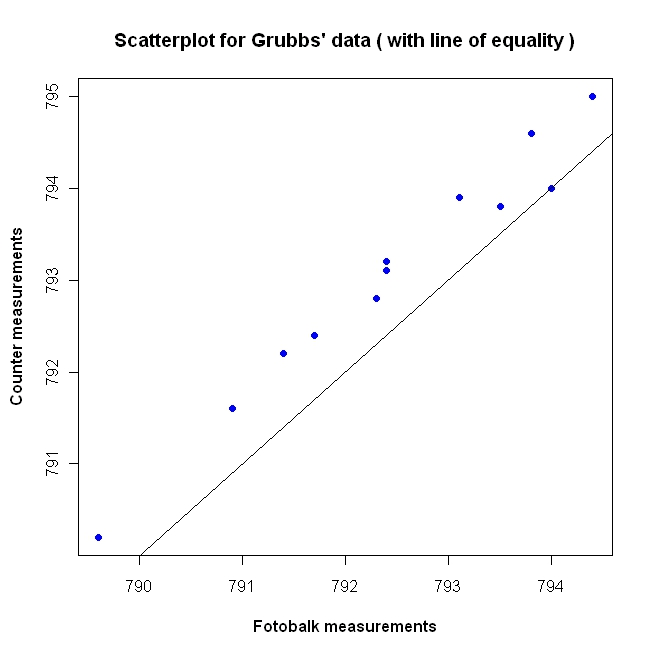
\includegraphics[width=130mm]{GrubbsScatter.jpeg}
  \caption{Scatter plot For Fotobalk and Counter Methods}\label{GrubbsScatter}
\end{center}
\end{figure}

In light of shortcomings associated with scatterplots, \citet*{BA83} recommend a further analysis of the data. Firstly
differences of measurements of two methods on the same subject should  be calculated, and then the average of those measurements
(Table 1.1). The averages of the two measurements is considered by Bland and Altman to the best estimate for the unknown true value.
Importantly both methods must measure with the same units. These  results are then plotted, with differences on the ordinate and
averages on the abscissa (figure 1.2).

The dashed line in figure 1.2 alludes to the inter method bias between the two methods, as mentioned previously. Bland and Altman
recommend the estimation of inter method bias by calculating the average of the differences. In the case of Grubbs data the inter
method bias is $-0.61$ metres per second.
\newpage
% latex table generated in R 2.6.0 by xtable 1.5-5 package
% Thu Aug 27 16:31:52 2009
\begin{table}[tbh]
\begin{center}

\begin{tabular}{|c|c|c|c|c|}
  \hline
 Round & Fotobalk [F] & Counter [C] & Differences [F-C] & Averages [(F+C)/2] \\
  \hline
1 & 793.80 & 794.60 & -0.80 & 794.20 \\
  2 & 793.10 & 793.90 & -0.80 & 793.50 \\
  3 & 792.40 & 793.20 & -0.80 & 792.80 \\
  4 & 794.00 & 794.00 & 0.00 & 794.00 \\
  5 & 791.40 & 792.20 & -0.80 & 791.80 \\
  6 & 792.40 & 793.10 & -0.70 & 792.80 \\
  7 & 791.70 & 792.40 & -0.70 & 792.00 \\
  8 & 792.30 & 792.80 & -0.50 & 792.50 \\
  9 & 789.60 & 790.20 & -0.60 & 789.90 \\
  10 & 794.40 & 795.00 & -0.60 & 794.70 \\
  11 & 790.90 & 791.60 & -0.70 & 791.20 \\
  12 & 793.50 & 793.80 & -0.30 & 793.60 \\
   \hline
\end{tabular}
\caption{Fotobalk and Counter Methods: Differences and Averages}
\end{center}
\end{table}

\begin{figure}[h!]
\begin{center}
  \includegraphics[width=120mm]{GrubbsBAplot.jpeg}
  \caption{Bland Altman plot for Fotobalk and Counter methods}\label{GrubbsBA}
\end{center}
\end{figure}
\newpage

From a visual inspection of Bland-Altman plot, it is also possible to compare the precision of each method in addition to the
inter-method bias.  Evidently the data points in the figure 1.2 tend to cluster near the bias line, particularly at the lower end
of the range of measurements. The variances of the differences seem to increase along the range. In case of small data sets, any
decision on the level of precision is subjective.

\subsection{Inspecting the Data}
Bland-Altman plots are a powerful graphical methodology for making a visual assessment of the data. \citet*{BA83} express the
motivation for this plot thusly:
\begin{quote}
"From this type of plot it is much easier to assess the magnitude of disagreement (both error and bias), spot outliers, and see
whether there is any trend, for example an increase in (difference) for high values. This way of plotting the data is a
very powerful way of displaying the results of a method comparison study."
\end{quote}


Figures XX YY and ZZ are three Bland-Altman plots derived from simulated data, each for the purpose of demonstrating how the plot
would inform an analyst of trends that would adversely affect use of the recommended methodology. Figure XX demonstrates how the
Bland Altman plot would indicate increasing variance of differences over the measurement range.

Figure ZZ is an example of cases where the inter-method bias changes over the measurement range. This is known as proportional
bias \citep{ludbrook97}.

\newpage
\begin{figure}[h!]
\begin{center}
  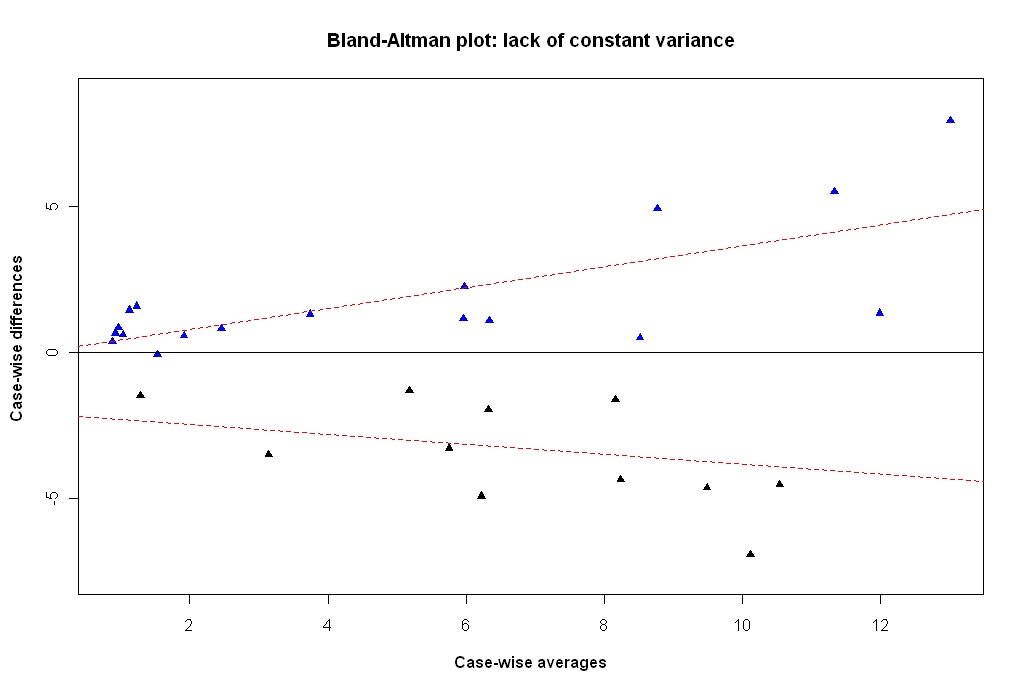
\includegraphics[width=125mm]{BAFanEffect.jpeg}
  \caption{Bland-Altman Plot demonstrating the increase of variance over the range}\label{BAFanEffect}
\end{center}
\end{figure}

\begin{figure}[h!]
\begin{center}
  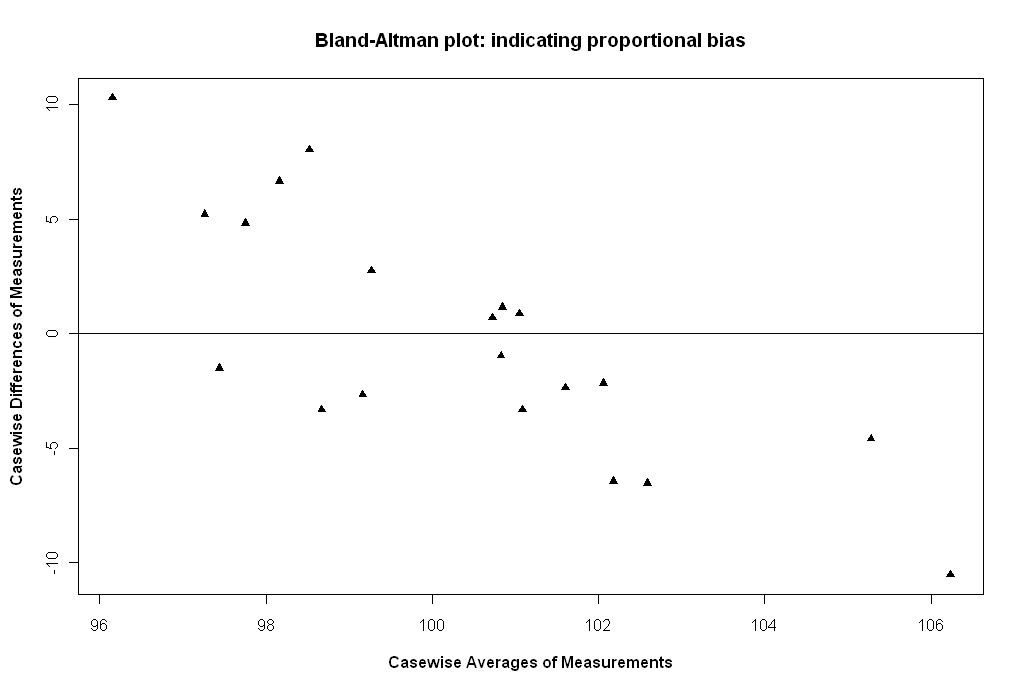
\includegraphics[width=125mm]{PropBias.jpeg}
  \caption{Bland-Altman Plot indicating the presence of proportional bias}\label{PropBias}
\end{center}
\end{figure}

\newpage
Figure ZZ is an example of cases where the inter-method bias changes over the measurement range. This is known as proportional
bias (Ludbrook, 1997). Both of these cases violate the assumptions necessary for further analysis using limits of agreement ,which
shall be discussed later. The plot also can be used to identify outliers. An outlier is an observation that is numerically distant
from the rest of the data. Classification thereof is a subjective decision in any analysis, but must be informed by the logic of the
formulation. Figure YY is a Bland Altman plot with two conspicuous observations, at the extreme left and right of the plot
respectively.


\begin{figure}[h!]
\begin{center}
  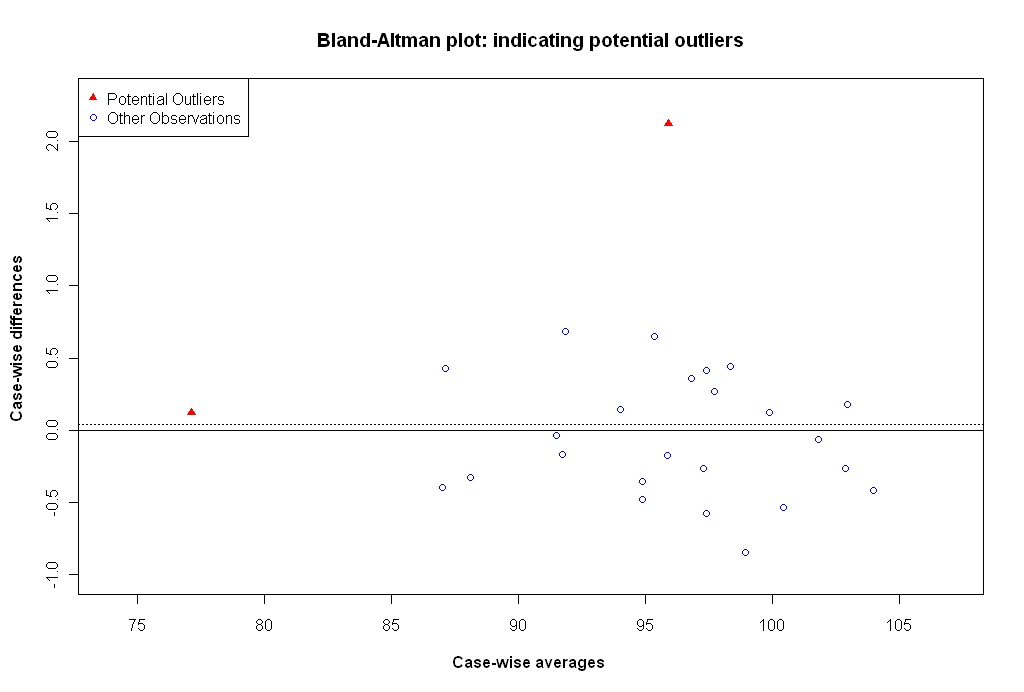
\includegraphics[width=125mm]{BAOutliers.jpeg}
  \caption{Bland-Altman Plot indicating the presence of Outliers}\label{PropBias}
\end{center}
\end{figure}

In the Bland-Altman plot, the horizontal displacement of any observation is supported by two independent measurements. Hence
any observation , such as the one on the extreme right of figure YY, should not be considered an outlier on the basis of a
noticeable horizontal displacement from the main cluster. The one on the extreme left should be considered an outlier, as it has a
noticeable vertical displacement from the rest of the observations.

\citet*{BA99} do not recommend excluding outliers from analyses. However recalculation of the inter-method bias estimate , and
further calculations based upon that estimate, are useful for assessing the influence of outliers.\citep{BA99} states that
\emph{"We usually find that this method of analysis is not too sensitive to one or two large outlying differences."}

\subsection{Limits of Agreement}
\citet{BA86} introduces an elaboration of the plot, adding to the plot `limits of agreement' to the plot. These limits are based
upon the standard deviation of the differences. The discussion shall be reverted to these limits of agreement in due course.

\subsection{Variations of the Bland Altman Plot}
\citet{BA99} remarks that it is possible to ignore the issue altogether, but the limits of agreement would wider apart than
necessary when just lower magnitude measurements are considered. Conversely the limits would be too narrow should only higher
magnitude measurements be used. To address the issue, they propose the logarithmic transformation of the data. The plot is then
formulated as the difference of paired log values against their mean. \citet{BA99} acknowledge that this is not easy to interpret,
and that it is not suitable in all cases.

\citet{BA99} offers two variations of the Bland -Altman plot that are intended to overcome potential problems that the conventional
plot would inappropriate for.

The first variation is a plot of casewise differences as percentage of averages, and is appropriate when there is an
increase in variability of the differences as the magnitude increases.


% When selecting this option the differences will be expressed as
% percentage of the averages. This option is useful when there is an
% increase in variability of the differences as the magnitude of the
% measurement increases.
\chapter{The Bland Altman Plot}
\section{Bland Altman Plots}
The issue of whether two measurement methods are comparable to the extent that they can be used interchangeably with sufficient
accuracy is encountered frequently in scientific research. Historically comparison of two methods of measurement was carried
out by use of matched pairs correlation coefficients or simple linear regression. Bland and Altman recognized the inadequacies of
these analyses and articulated quite thoroughly the basis on which of which they are unsuitable for comparing two methods of
measurement \citep*{BA83}.

As an alternative they proposed a simple statistical methodology specifically appropriate for method comparison studies. They
acknowledge that there are other valid methodologies, but argue that a simple approach is preferable to complex approaches,
\emph{"especially when the results must be explained to non-statisticians"} \citep*{BA83}.

The first step recommended which the authors argue should be mandatory is construction of a simple scatter plot of the data.
The line of equality ($X=Y$) should also be shown, as it is necessary to give the correct interpretation of how both methods
compare. A scatter plot of the Grubbs data is shown in figure 2.1. A visual inspection thereof confirms the previous conclusion that
there is an inter method bias present, i.e. Fotobalk device has a tendency to record a lower velocity.

\begin{figure}[h!]
\begin{center}
  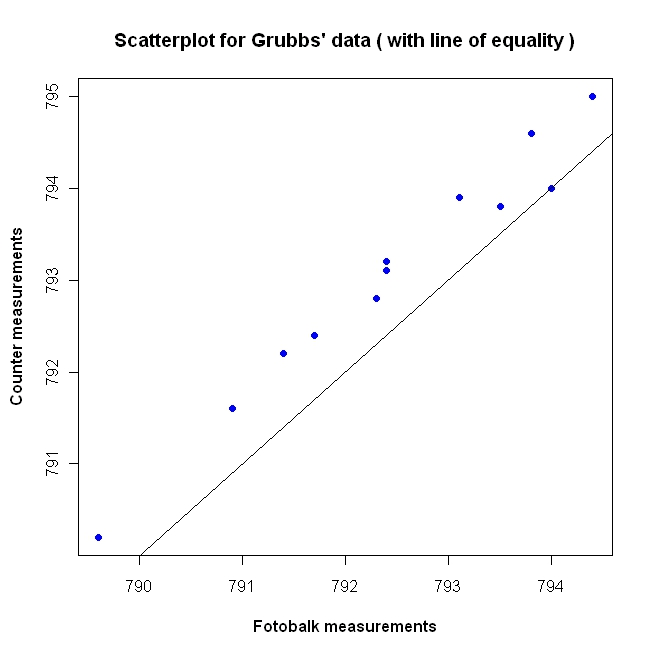
\includegraphics[width=130mm]{GrubbsScatter.jpeg}
  \caption{Scatter plot For Fotobalk and Counter Methods}\label{GrubbsScatter}
\end{center}
\end{figure}

In light of shortcomings associated with scatterplots,
\citet*{BA83} recommend a further analysis of the data. Firstly differences of measurements of two methods on the same subject
should  be calculated, and then the average of those measurements (Table 1.1). The averages of the two measurements is considered by
Bland and Altman to the best estimate for the unknown true value. Importantly both methods must measure with the same units. These
results are then plotted, with differences on the ordinate and averages on the abscissa (figure 1.2). \citet*{BA83}express the
motivation for this plot thusly:
\begin{quote}
"From this type of plot it is much easier to assess the magnitude of disagreement (both error and bias), spot outliers, and see
whether there is any trend, for example an increase in (difference) for high values. This way of plotting the data is a
very powerful way of displaying the results of a method comparison
study."
\end{quote}
\newpage
% latex table generated in R 2.6.0 by xtable 1.5-5 package
% Thu Aug 27 16:31:52 2009
\begin{table}[tbh]
\begin{center}

\begin{tabular}{|c|c|c|c|c|}
  \hline
 Round & Fotobalk [F] & Counter [C] & Differences [F-C] & Averages [(F+C)/2] \\
  \hline
1 & 793.80 & 794.60 & -0.80 & 794.20 \\
  2 & 793.10 & 793.90 & -0.80 & 793.50 \\
  3 & 792.40 & 793.20 & -0.80 & 792.80 \\
  4 & 794.00 & 794.00 & 0.00 & 794.00 \\
  5 & 791.40 & 792.20 & -0.80 & 791.80 \\
  6 & 792.40 & 793.10 & -0.70 & 792.80 \\
  7 & 791.70 & 792.40 & -0.70 & 792.00 \\
  8 & 792.30 & 792.80 & -0.50 & 792.50 \\
  9 & 789.60 & 790.20 & -0.60 & 789.90 \\
  10 & 794.40 & 795.00 & -0.60 & 794.70 \\
  11 & 790.90 & 791.60 & -0.70 & 791.20 \\
  12 & 793.50 & 793.80 & -0.30 & 793.60 \\
   \hline
\end{tabular}
\caption{Fotobalk and Counter Methods: Differences and Averages}
\end{center}
\end{table}

The dashed line in figure 1.2 alludes to the inter method bias
between the two methods, as mentioned previously. Bland and Altman
recommend the estimation of inter method bias by calculating the
average of the differences. In the case of Grubbs data the inter
method bias is $-0.61$ metres per second.
\newpage
\begin{figure}[h!]
\begin{center}
  \includegraphics[width=120mm]{GrubbsBAplot.jpeg}
  \caption{Bland Altman plot for Fotobalk and Counter methods}\label{GrubbsBA}
\end{center}
\end{figure}

From a visual inspection of Bland-Altman plot, it is also possible
to compare the precision of each method in addition to the
inter-method bias.  Evidently the data points in the figure HH
tend to cluster near the bias line, particularly at the lower end
of the range of measurements. The variances of the differences
seem to increase along the range. In case of small data sets, Any
decision on the level of precision is subjective.

Figures XX and ZZ are Bland-Altman plots of data simulated for
expository purposes. Figure XX demonstrates how the Bland Altman
plot would indicate increasing variance of differences over the
measurement range. Figure ZZ is an example of cases where the
inter-method bias changes over the measurement range. This is
known as proportional bias \citep{ludbrook97}.

\newpage
\begin{figure}[h!]
\begin{center}
  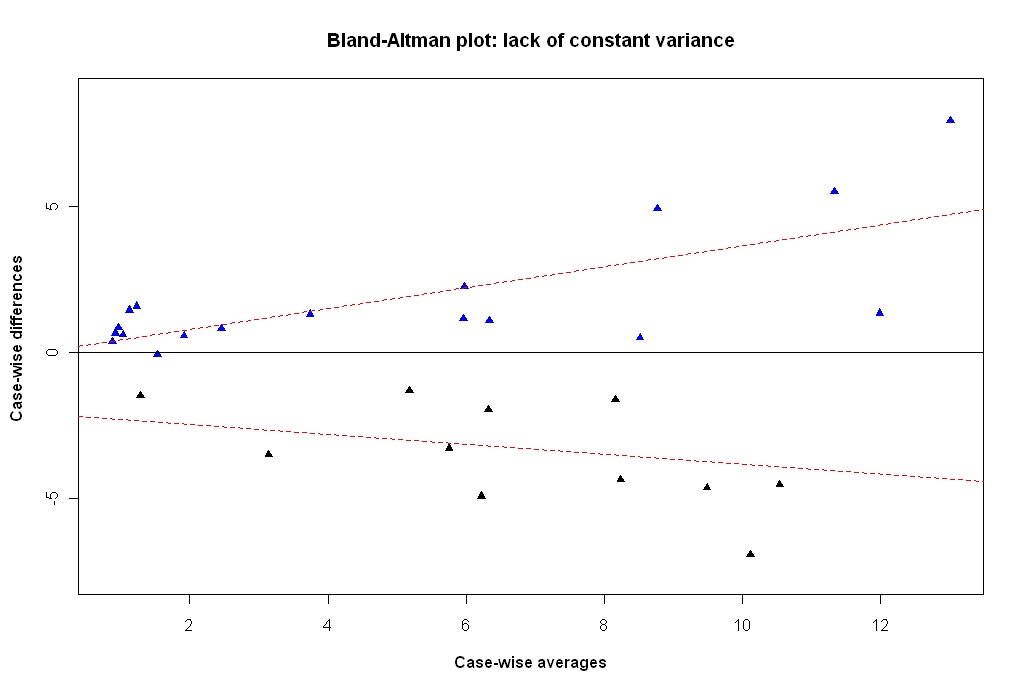
\includegraphics[width=125mm]{BAFanEffect.jpeg}
  \caption{Bland-Altman Plot demonstrating the increase of variance over the range}\label{BAFanEffect}
\end{center}
\end{figure}
\begin{figure}[h!]
\begin{center}
  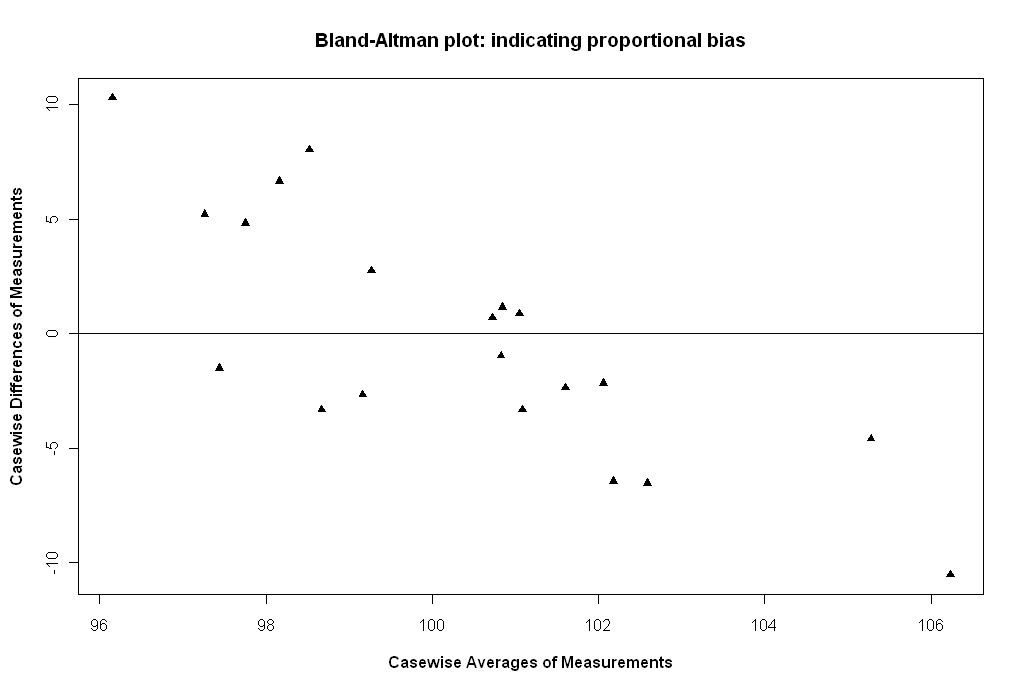
\includegraphics[width=125mm]{PropBias.jpeg}
  \caption{Bland-Altman Plot indicating the presence of proportional bias}\label{PropBias}
\end{center}
\end{figure}
\newpage



The fourth pair of measurements from table 1.1 show both methods
recording the same value, hence the difference is zero. In
assessing the impact of the corresponding data point, two
conflicting conclusions can be drawn.

One conclusion is that it is an outlier, and the precision of the
differences is consistent along the range of measurements. The
other conclusion is that is not an outlier, and the precision
increases proportionately along the range of measurements.

The Bland Altman plot is a simple tool for inspection of the data,
but in itself it offers no formal testing procedure in this
regard. To this end, the approach proposed by \citet{BA83} is a
formal test on the Pearson correlation coefficient  of casewise
differences and means ($\rho_{AD}$). According to the authors,
this test is equivalent to a well established tests for equality
of variances, known as the `Pitman Morgan Test' \citep{Pitman,
Morgan}.

For the Grubbs data, the correlation coefficient estimate
($r_{AD}$) is 0.2625, with a 95\% confidence interval of (-0.366,
0.726) estimated by Fishers 'r to z' transformation \citep{Cohen}.
The null hypothesis ($\rho_{AD}$ =0) would fail to be rejected.
Consequently the null hypothesis of equal variances of each method
would also fail to be rejected.

There has no been no further mention of this particular test in
the subsequent article published by Bland and Altman, although
\citet{BA99} refers to Spearmans' rank correlation coefficient.

The second variation is a plot of casewise ratios as percentage of
averages.

% Plot ratios When this option is selected then the ratios of the
% measurements will be plotted instead of the differences (avoiding
% the need for log transformation). This option as well is useful
% when there is an increase in variability of the differences as the
% magnitude of the measurement increases.


\subsection{Formal Testing}
The Bland Altman plot is a simple tool for inspection of the data,
but in itself it offers no formal testing procedure in this
regard. To this end, the approach proposed by \citet{BA83} is a
formal test on the Pearson correlation coefficient  of casewise
differences and means ($\rho_{AD}$). According to the authors,
this test is equivalent to a well established tests for equality
of variances, known as the `Pitman Morgan Test' \citep{Pitman,
Morgan}.

For the Grubbs data, the correlation coefficient estimate
($r_{AD}$) is 0.2625, with a 95\% confidence interval of (-0.366,
0.726) estimated by Fishers 'r to z' transformation \citep{Cohen}.
The null hypothesis ($\rho_{AD}$ =0) would fail to be rejected.
Consequently the null hypothesis of equal variances of each method
would also fail to be rejected.

There has no been no further mention of this particular test in
the subsequent article published by Bland and Altman, although
\citet{BA99} refers to Spearmans' rank correlation coefficient.

\section{Bland Altman plot and the Treatment of Outliers}
We wish to determine how outliers should be treated in a Bland
Altman Plot.In their 1983 paper Bland and Altman  merely state
that the plot can be used to 'spot outliers'. However they pay
more attention to the issue of outliers in their $1986$ paper,
wherein they present a data set with an extreme outlier.

\section{Bland Altman Plots}
The issue of whether two measurement methods are comparable to the
extent that they can be used interchangeably with sufficient
accuracy is encountered frequently in scientific research.
Historically comparison of two methods of measurement was carried
out by use of matched pairs correlation coefficients or simple
linear regression. Bland and Altman recognized the inadequacies of
these analyses and articulated quite thoroughly the basis on which
of which they are unsuitable for comparing two methods of
measurement \citep*{BA83}.

As an alternative they proposed a simple statistical methodology
specifically appropriate for method comparison studies. They
acknowledge that there are other valid methodologies, but argue
that a simple approach is preferable to complex approaches,
\emph{"especially when the results must be explained to
non-statisticians"} \citep*{BA83}.

The first step recommended which the authors argue should be
mandatory is construction of a simple scatter plot of the data.
The line of equality ($X=Y$) should also be shown, as it is
necessary to give the correct interpretation of how both methods
compare. A scatter plot of the Grubbs data is shown in figure 2.1.
A visual inspection thereof confirms the previous conclusion that
there is an inter method bias present, i.e. Fotobalk device has a
tendency to record a lower velocity.



In light of shortcomings associated with scatterplots,
\citet*{BA83} recommend a further analysis of the data. Firstly
differences of measurements of two methods on the same subject
should  be calculated, and then the average of those measurements
(Table 1.1). The averages of the two measurements is considered by
Bland and Altman to the best estimate for the unknown true value.
Importantly both methods must measure with the same units. These
results are then plotted, with differences on the ordinate and
averages on the abscissa (figure 1.2). \citet*{BA83}express the
motivation for this plot thusly:
\begin{quote}
"From this type of plot it is much easier to assess the magnitude
of disagreement (both error and bias), spot outliers, and see
whether there is any trend, for example an increase in
(difference) for high values. This way of plotting the data is a
very powerful way of displaying the results of a method comparison
study."
\end{quote}
\newpage
% latex table generated in R 2.6.0 by xtable 1.5-5 package
% Thu Aug 27 16:31:52 2009
\begin{table}[tbh]
\begin{center}

\begin{tabular}{|c|c|c|c|c|}
  \hline
 Round & Fotobalk [F] & Counter [C] & Differences [F-C] & Averages [(F+C)/2] \\
  \hline
1 & 793.80 & 794.60 & -0.80 & 794.20 \\
  2 & 793.10 & 793.90 & -0.80 & 793.50 \\
  3 & 792.40 & 793.20 & -0.80 & 792.80 \\
  4 & 794.00 & 794.00 & 0.00 & 794.00 \\
  5 & 791.40 & 792.20 & -0.80 & 791.80 \\
  6 & 792.40 & 793.10 & -0.70 & 792.80 \\
  7 & 791.70 & 792.40 & -0.70 & 792.00 \\
  8 & 792.30 & 792.80 & -0.50 & 792.50 \\
  9 & 789.60 & 790.20 & -0.60 & 789.90 \\
  10 & 794.40 & 795.00 & -0.60 & 794.70 \\
  11 & 790.90 & 791.60 & -0.70 & 791.20 \\
  12 & 793.50 & 793.80 & -0.30 & 793.60 \\
   \hline
\end{tabular}
\caption{Fotobalk and Counter Methods: Differences and Averages}
\end{center}
\end{table}

The dashed line in figure 1.2 alludes to the inter method bias
between the two methods, as mentioned previously. Bland and Altman
recommend the estimation of inter method bias by calculating the
average of the differences. In the case of Grubbs data the inter
method bias is $-0.61$ metres per second.


From a visual inspection of Bland-Altman plot, it is also possible
to compare the precision of each method in addition to the
inter-method bias.  Evidently the data points in the figure HH
tend to cluster near the bias line, particularly at the lower end
of the range of measurements. The variances of the differences
seem to increase along the range. In case of small data sets, Any
decision on the level of precision is subjective.

Figures XX and ZZ are Bland-Altman plots of data simulated for
expository purposes. Figure XX demonstrates how the Bland Altman
plot would indicate increasing variance of differences over the
measurement range. Figure ZZ is an example of cases where the
inter-method bias changes over the measurement range. This is
known as proportional bias \citep{ludbrook97}.




The fourth pair of measurements from table 1.1 show both methods
recording the same value, hence the difference is zero. In
assessing the impact of the corresponding data point, two
conflicting conclusions can be drawn.

One conclusion is that it is an outlier, and the precision of the
differences is consistent along the range of measurements. The
other conclusion is that is not an outlier, and the precision
increases proportionately along the range of measurements.

The Bland Altman plot is a simple tool for inspection of the data,
but in itself it offers no formal testing procedure in this
regard. To this end, the approach proposed by \citet{BA83} is a
formal test on the Pearson correlation coefficient  of casewise
differences and means ($\rho_{AD}$). According to the authors,
this test is equivalent to a well established tests for equality
of variances, known as the `Pitman Morgan Test' \citep{Pitman,
Morgan}.

For the Grubbs data, the correlation coefficient estimate
($r_{AD}$) is 0.2625, with a 95\% confidence interval of (-0.366,
0.726) estimated by Fishers 'r to z' transformation \citep{Cohen}.
The null hypothesis ($\rho_{AD}$ =0) would fail to be rejected.
Consequently the null hypothesis of equal variances of each method
would also fail to be rejected.

There has no been no further mention of this particular test in
the subsequent article published by Bland and Altman, although
\citet{BA99} refers to Spearmans' rank correlation coefficient.

\subsection{Criticism of Bland Altman Plot}
Hopkins[$8$] argues that the plot indicates incorrectly that there
are systematic differences or bias in the relationship between two
measures, when one has been calibrated against the other.
\\
An Evaluation of the correlation between the difference and means
complement the analysis.
\\
Bland and Altman caution that the calculations are based on the
assumption that the data is normally distributed. This can be
verified by using a histogram. If Data is not normally
distributed, it can be transformed.
\section{Bland Altman plot and the Treatment of Outliers}
We wish to determine how outliers should be treated in a Bland
Altman Plot.In their 1983 paper Bland and Altman  merely state
that the plot can be used to 'spot outliers'. However they pay
more attention to the issue of outliers in their $1986$ paper,
wherein they present a data set with an extreme outlier.
\\
In Bland and Altman's 1999 paper, we get the clearest indication
of what Bland and Altman suggest on how to react to the presence
of outliers. Their recommendation is to recalculate the limits
without them, in order to test the difference with the calculation
where outliers are retained. \emph{The span has reduced from 77 to
59 mmHg, a noticeable but not particularly large reduction.}
However, they do not recommend removing outliers. Furthermore,
they say: \emph{We usually find that this method of analysis is
not too sensitive to one or two large outlying differences.}
\\
\\
In  their $1986$ paper, Bland and Altman give an example of an
outlier. They state that it could be omitted in practice, but make
no further comments on the matter.
\\
We ask if this would be so in all cases. Given that the limits of
agreement may or may not be disregarded, depending on their
perceived suitability, we examine whether it would possible that
the deletion of an outlier may lead to a calculation of limits of
agreement that are usable in all cases?
\\
\\
Should an Outlying Observation be omitted from a data set? In
general, this is not considered prudent. Also, it may be required
that the outliers are worthy of particular attention themselves.
\section{Variations of the Bland Altman Plot}
\citet{BA99} offers two variations of the Bland -Altman plot that
are intended to overcome potential problems that the conventional
plot would inappropriate for.

The first variation is a plot of casewise differences as
percentage of averages, and is appropriate when there is an
increase in variability of the differences as the magnitude
increases.


% When selecting this option the differences will be expressed as
% percentage of the averages. This option is useful when there is an
% increase in variability of the differences as the magnitude of the
% measurement increases.


The second variation is a plot of casewise ratios as percentage of
averages.

% Plot ratios When this option is selected then the ratios of the
% measurements will be plotted instead of the differences (avoiding
% the need for log transformation). This option as well is useful
% when there is an increase in variability of the differences as the
% magnitude of the measurement increases.

%%%%%%%%%%%%%%%%%%%%%%%%%%%%%%%%%%%%%%%%%%%%%%%%%%%%%%%%%%%%%%%%%%%%%%%%%%%%%%%%%%%%%%%%%%%%%%%%%%%%%%%%%%%%%%%%%%%%%%%%
\newpage








\subsubsection{Classifying outliers and recalculating} We opted to
examine this matter in more detail. The following points have to
be considered:
\\
 \indent How to suitably identify an outlier (in a generalized sense)
\\
\indent Would a recalculation of the limits of agreement generally
results in  a compacted range between the upper and lower limits
of agreement?
\addcontentsline{toc}{section}{Bibliography}

\bibliography{transferbib}
\end{document}
